\documentclass[12pt]{article}

\usepackage{graphicx}
\usepackage{listings}
\usepackage{hyperref}
\usepackage{float}
\usepackage{enumitem}

\graphicspath{ {./images/} }

\oddsidemargin 0mm
\evensidemargin 0mm
\textwidth 160mm
\textheight 200mm

\pagestyle {plain}
\pagenumbering{arabic}

\newcounter{stepnum}

\title{CS/SE 2XC3 Lab 8 Report}
\author{
  Glotov, Oleg\\ L03, 400174037\\
  \texttt{glotovo@mcmaster.ca}
  \and
  Willson, Emma\\ L02, 400309856\\
  \texttt{willsone@mcmaster.ca}
  }
\date{\today}

\begin{document}

\maketitle

This report includes the main observations that we found in this week's lab, along with the analysis of our results.

\newpage 
\section{Prim's Algorithm}
In this section, we discuss Prim's algorithm for finding the minimum spanning tree. 
\subsection{Prim's Algorithm Version 1}
In this implementation of Prim’s algorithm, two sets are used: One set contains a list of vertices already included in MST, the other set contains vertices not yet included. With an adjacency list representation, all graph vertices can be traversed in O(V+E) time using BFS. Here, the vertices not yet included in the MST will be stored in a list that has to be sorted each time. This approach is inefficient and will is improved in the following implementation.
\subsection{List vs. Min Heap}
The most expensive functions in the implementation of Prim's algorithm are finding and updating the weight of the minimum edge. Our first implementation uses a list of edges that are sorted by weight. The algorithm re-sorts this list for every edge visited. The Python \verb+sort()+ function has a time complexity in $O(nlogn)$. Our second implementation uses a heap of nodes that are sorted by edge weight. The heap property is maintained using \verb+extract_min+ and \verb+decrease_key+, so there is no need to sort. Both of these functions are in $O(logn)$ The difference between these implementations is that the first one visits each edge, while the second visits each node. As the graph becomes more densely connected, visiting nodes (v2) becomes less efficient than visiting edges (v1). However in a sparse graph with a large number of nodes, using a min heap of nodes is faster. That's why we expect v2 to perform significantly better on large, sparse graphs.
\begin{figure}[H]
\centering
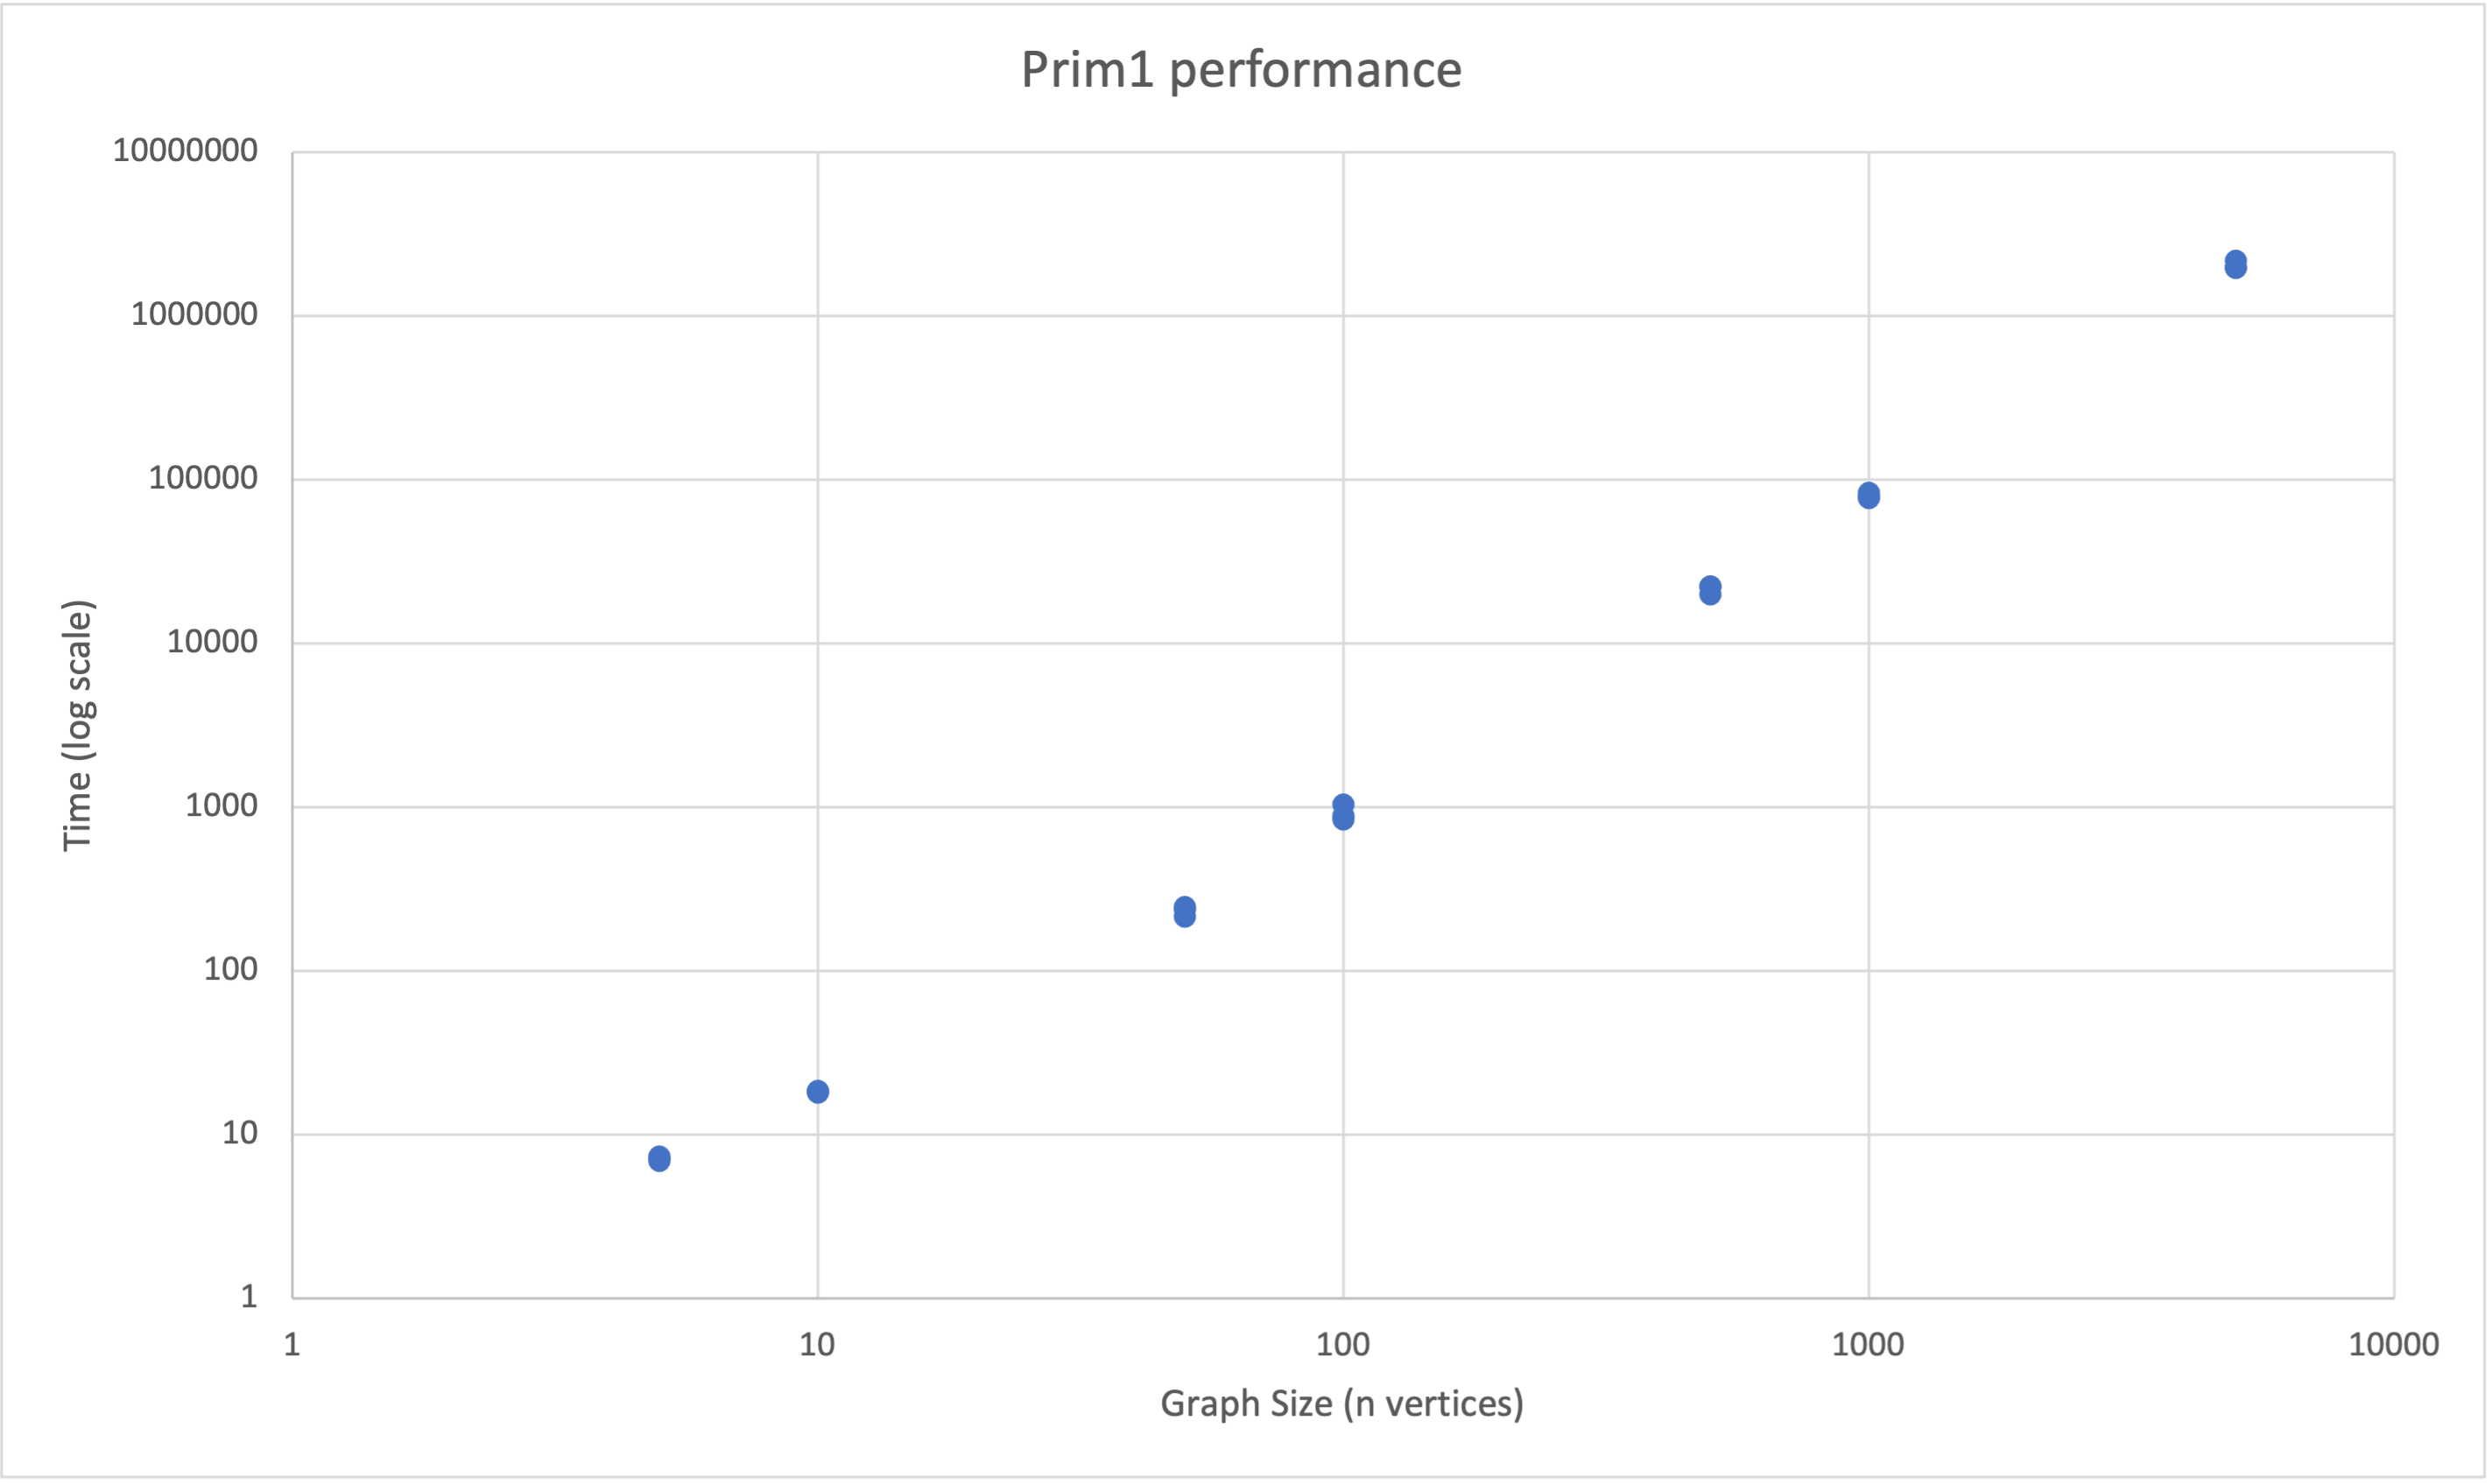
\includegraphics[width=0.7\textwidth,height=\textheight,keepaspectratio]{prim1.png}
\caption{time complexity of prim v1 vs. prim v2}
\label{Figure: m1}
\end{figure}
\noindent As shown in the graph above, ... 

\end{document}

